\clearpage

\section{Transparent with 1+1 Protection - Reference Network}
In this case study we focus on the transparent case with 1 + 1 protection for the reference network.

\subsection{Physical Network Topology}
\begin{tcolorbox}	
\begin{tabular}{p{2.75cm} p{0.2cm} p{10.5cm}} 	
\textbf{Student Name}  &:& Tiago Esteves    (October 03, 2017 - )\\
\end{tabular}
\end{tcolorbox}

In the figure below we ca see that our reference network is the same as in the subsection \ref{Reference_Network_Transp}.

\begin{figure}[h!]
\centering
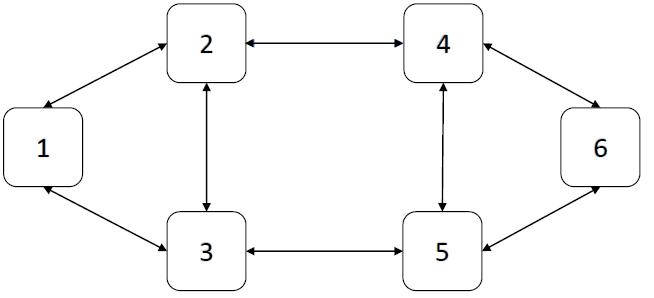
\includegraphics[width=\textwidth]{RedeTeste}
\caption{Physical Topology of the Reference Network.}
\end{figure}

The average length of the links, matrix of distances between the respective nodes and the ODU's matrices is the same as in the subsection \ref{Reference_Network_Transp_Topology} the same happens for the total network traffic for the two scenarios.\\

Finally for this case has to take into consideration the table \ref{table_ref_net_transp} once again.


\subsection{Dimensioning using ILP}
\begin{tcolorbox}	
\begin{tabular}{p{2.75cm} p{0.2cm} p{10.5cm}} 	
\textbf{Student Name}  &:& Tiago Esteves    (October 03, 2017 - )\\
\end{tabular}
\end{tcolorbox}


In this section we will do the dimensioning of the network mentioned in the previous section to calculate the value of your CAPEX, for this we will use the ILP model describe in section \ref{ILP_Transp_Protection} and we can get the best possible solution.
For this we will use MATLAB which is ideal for dealing with linear programming problems and can call the LPsolve through an external interface.
The network cost and all the formulas used in this section are the same used in subsection \ref{Net_Costs_Transp} as such if only we will mention one subsection where with the results obtained through the described model.\\


\textbf{Scenario 1: Reference Network Low Traffic} \label{Scenario1_transp} \\

In this scenario we used the table \ref{table_ref_net_transp}. In the table \ref{result_ILP1_TP} we can see the values calculated through MatLab and using the values indicated in table \ref{table_cost_transp} we can finally calculate the CAPEX value. \\

Using equation \ref{linkCostsTransp} : \\
$C_L$ = $($2 * 15 000 * 8$)$ + $($2 * 5 000 * 100 * 26 $)$ + $($24 * 4 000$)$ \\
$C_L$ = \textbf{26 336 000 \euro} \\

Using equation \ref{electricalCostTransp} : \\
$C_{exc}$ = $($6 * 10 000$)$ + 1 000 * $($2 * 1 000$)$ \\
$C_{exc}$ = \textbf{2 060 000\euro} \\

Using equation \ref{opticalCost} : \\
$C_{oxc}$ = $($6 * 10 000$)$ + 1 000 * $($ 34 + 52 $)$ \\
$C_{oxc}$ = \textbf{146 000 \euro} \\
$C_N$ = $C_{oxc}$ + $C_{exc}$ = \textbf{2 206 000 \euro} \\

$CAPEX$ = 26 336 000 + 2 206 000 = \textbf{28 542 000 \euro}\\

\begin{table}[h!]
\centering
\begin{tabular}{|| c | c || c | c || c | c ||}
 \hline
 Number of optical channels & Value & ADD PORTS & Value & LINE PORTS & Value \\
 \hline\hline
 in the link (1,2) & 3 & Node 1 & 5 & Node 1 & 5 \\
 in the link (1,3) & 2 & Node 2 & 6 & Node 2 & 12 \\
 in the link (2,3) & 3 & Node 3 & 5 & Node 3 & 9 \\
 in the link (2,4) & 6 & Node 4 & 5 & Node 4 & 11 \\
 in the link (3,5) & 4 & Node 5 & 6 & Node 5 & 8 \\
 in the link (4,5) & 1 & Node 6 & 7 & Node 6 & 7 \\
 in the link (4,6) & 4 & & & & \\
 in the link (5,6) & 3 & & & & \\
 \hline
\end{tabular}
\caption{Table with results for scenario 1}
\label{result_ILP1_TP}
\end{table}


\textbf{Scenario 2: Reference Network High Traffic} \label{Scenario2_transp} \\

In this scenario we used again the table \ref{table_ref_net_transp} In the table \ref{result_ILP2_TP} we can see the values calculated through MatLab and using the values indicated in table \ref{table_cost_transp} we can finally calculate the CAPEX value.\\

\begin{table}[h!]
\centering
\begin{tabular}{|| c | c || c | c || c | c ||}
 \hline
 Number of optical channels & Value & ADD PORTS & Value & LINE PORTS & Value \\
 \hline\hline
 in the link (1,2) & 7 & Node 1 & 11 & Node 1 & 11 \\
 in the link (1,3) & 4 & Node 2 & 25 & Node 2 & 37 \\
 in the link (2,3) & 8 & Node 3 & 16 & Node 3 & 22 \\
 in the link (2,4) & 22 & Node 4 & 8 & Node 4 & 42 \\
 in the link (3,5) & 10 & Node 5 & 23 & Node 5 & 25 \\
 in the link (4,5) & 2 & Node 6 & 31 & Node 6 & 31 \\
 in the link (4,6) & 18 & & & & \\
 in the link (5,6) & 13 & & & & \\
 \hline
\end{tabular}
\caption{Table with results for scenario 2}
\label{result_ILP2_TP}
\end{table}


Using equation \ref{linkCostsTransp} : \\
$C_L$ = $($2 * 15 000 * 8$)$ + $($2 * 5 000 * 100 * 84 $)$ + $($24 * 4 000$)$ \\
$C_L$ = \textbf{84 240 000 \euro} \\

Using equation \ref{electricalCostTransp} : \\
$C_{exc}$ = $($6 * 10 000$)$ + 1 000 * $($2 * 10 000$)$ \\
$C_{exc}$ = \textbf{20 060 000 \euro} \\

Using equation \ref{opticalCost} : \\
$C_{oxc}$ = $($6 * 10 000$)$ + 1 000 * $($114 + 168$)$ \\
$C_{oxc}$ = \textbf{342 000 \euro} \\
$C_N$ = $C_{oxc}$ + $C_{exc}$ = \textbf{20 402 000 \euro} \\

$CAPEX$ = 84 240 000 + 20 402 000 = \textbf{104 642 000 \euro}\\


\subsection{Dimensioning using Heuristics}

\subsubsection{Heuristics Results}

\subsection{Comparative Analysis}


\newpage
\section{Transparent with 1+1 Protection - European Optical Network}

In this case study we focus on the transparent case with 1+1 protection for the realistic network.

\subsection{Physical Network Topology}
\begin{tcolorbox}	
\begin{tabular}{p{2.75cm} p{0.2cm} p{10.5cm}} 	
\textbf{Student Name}  &:& Tiago Esteves    (October 03, 2017 - )\\
\end{tabular}
\end{tcolorbox}

The real network chosen for this work is the EON (European Optical Network).

\begin{figure}[h!]
\centering
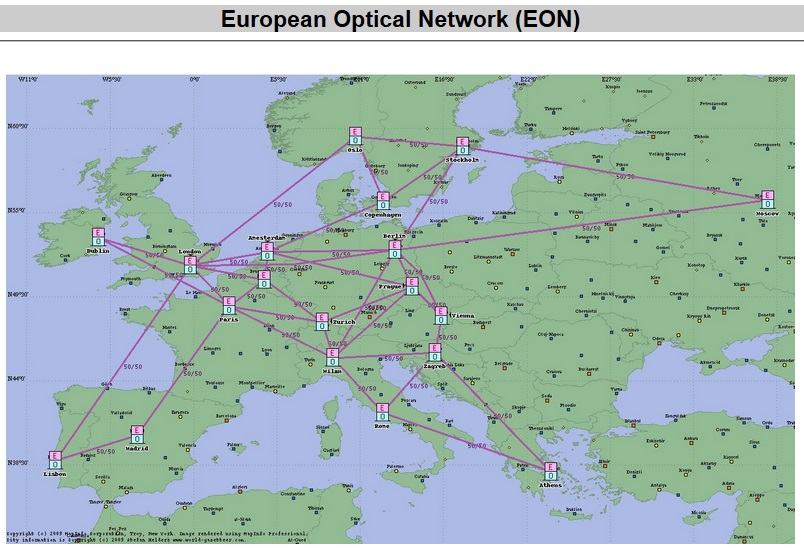
\includegraphics[width=\textwidth]{EON_Rede_Realista}
\caption{Physical topology of the realistic network.}
\end{figure}

Since the realistic network used in this case has already been mentioned previously in section \ref{Realistic_Network_Transp} we can assume that the table \ref{table_real_net_transp} is the same and the table \ref{city_nodes_realnet_transp} where each city contains a number of a node in the network also is the same.\\
The distance matrix constructed based on real distances between cities and the matrices of ODU's are also the same.
Finally, the total traffic for the two scenarios are:\\
Low Traffic: \textbf{2 TBits/s}; \quad High Traffic: \textbf{20 TBits/s};\\

\subsection{Dimensioning using ILP}
\begin{tcolorbox}	
\begin{tabular}{p{2.75cm} p{0.2cm} p{10.5cm}} 	
\textbf{Student Name}  &:& Tiago Esteves    (October 03, 2017 - )\\
\end{tabular}
\end{tcolorbox}

The initial subsection is the same as the subsection of the previous case so in this case it will be omitted presenting only the subsection of the results.
In this section we will do the dimensioning of the network mentioned in the previous section to calculate the value of your CAPEX, for this we will use the ILP model describe in section \ref{ILP_Transp_Protection}.
This real network consists of many nodes and with many links between them as such the lpsolve takes immense time to get an optimal solution. Therefore, in this case, the execution time was defined as being two days (48 hours) and after that time presented the best solution.\\

\textbf{Scenario 1: Realistic Network Low Traffic} \label{Scenario3_transp} \\

In this scenario we used the table \ref{table_real_net_transp} In the previous page we can see the table \ref{result_ILP3_TP} with the values calculated through MatLab and using the values indicated in table \ref{table_cost_transp} we can finally calculate the CAPEX value. \\

Using equation \ref{linkCostsTransp} : \\
$C_L$ = $($2 * 15 000 * 37$)$ + $($2 * 5 000 * 100 * 378$)$ + $($24 * 4 000$)$ \\
$C_L$ = \textbf{379 206 000 \euro} \\

Using equation \ref{electricalCostTransp} : \\
$C_{exc}$ = $($19 * 10 000$)$ + 1 000 * $($2 * 4 000$)$ \\
$C_{exc}$ = \textbf{8 190 000\euro} \\

Using equation \ref{opticalCost} : \\
$C_{oxc}$ = $($19 * 10 000$)$ + 1 000 * $($276 + 756$)$ \\
$C_{oxc}$ = \textbf{1 222 000 \euro} \\
$C_N$ = $C_{oxc}$ + $C_{exc}$ = \textbf{9 412 000 \euro} \\

$CAPEX$ = 379 206 000 + 9 412 000 = \textbf{388 618 000 \euro}\\

\begin{table}[h!]
\centering
\begin{tabular}{|| c | c || c | c || c | c ||}
 \hline
 Number of optical channels & Value & ADD PORTS & Value & LINE PORTS & Value \\
 \hline\hline
in link (1,2): & 15& Node 1 & 19 & Node 1 & 37 \\
in link (1,4): & 6& Node 2 & 19 & Node 2 & 51 \\
in link (1,15): & 16& Node 3 & 19 & Node 3 & 19 \\
in link (2,3): & 4& Node 4 & 19 & Node 4 & 23 \\
in link (2,4): & 10& Node 5 & 19 & Node 5 & 173 \\
in link (2,5): & 22& Node 6 & 19 & Node 6 & 29 \\
in link (3,5): & 15& Node 7 & 19 & Node 7 & 103 \\
in link (4,14): & 7& Node 8 & 19 & Node 8 & 43 \\
in link (5,6): & 10& Node 9 & 14 & Node 9 & 14 \\
in link (5,7): & 80& Node 10 & 11 & Node 10 & 11 \\
in link (5,11): & 22& Node 11 & 10 & Node 11 & 60 \\
in link (5,14): & 7& Node 12 & 11 & Node 12 & 17 \\
in link (5,15): & 17& Node 13 & 11 & Node 13 & 17 \\
in link (6,7): & 5& Node 14 & 9 & Node 14 & 23 \\
in link (6,11): & 4& Node 15 & 10 & Node 15 & 70 \\
in link (6,12): & 7& Node 16 & 10 & Node 16 & 10 \\
in link (6,14): & 3& Node 17 & 9 & Node 17 & 27 \\
in link (7,8): & 18& Node 18 & 10 & Node 18 & 10 \\
in link (8,9): & 12& Node 19 & 19 & Node 19 & 19 \\
in link (8,10): & 2& & & & \\
in link (8,11): & 11& & & & \\
in link (9,10): & 2& & & & \\
in link (10,11): & 7& & & & \\
in link (11,12): & 4& & & & \\
in link (11,17): & 12& & & & \\
in link (12,13): & 6& & & & \\
in link (12,17): & 0& & & & \\
in link (13,14): & 5& & & & \\
in link (13,15): & 5& & & & \\
in link (13,17): & 1& & & & \\
in link (14,15): & 1& & & & \\
in link (15,16): & 9& & & & \\
in link (15,17): & 5& & & & \\
in link (15,19): & 17& & & & \\
in link (16,17): & 1& & & & \\
in link (17,18): & 8& & & & \\
in link (18,19): & 2& & & & \\
\hline
\end{tabular}
\caption{Table with results  for scenario 1}
\label{result_ILP3_TP}
\end{table}

\newpage
\textbf{Scenario 4: Realistic Network High Traffic} \label{Scenario4_transp} \\

This scenario is identical to the previous one, therefore, the execution time was the same. In this scenario we used again the table \ref{table_real_net_transp} In the next page we can see the table \ref{result_ILP4_TP} with the values calculated through MatLab and using the values indicated in table \ref{table_cost_transp} we can finally calculate the CAPEX value. \\

Using equation \ref{linkCostsTransp} : \\
$C_L$ = $($2 * 15 000 * 37$)$ + $($2 * 5 000 * 100 * 572$)$ + $($24 * 4 000$)$ \\
$C_L$ = \textbf{573 206 000 \euro} \\

Using equation \ref{electricalCostTransp} : \\
$C_{exc}$ = $($19 * 10 000$)$ + 1 000 * $($2 * 40 000$)$ \\
$C_{exc}$ = \textbf{80 190 000\euro} \\

Using equation \ref{opticalCost} : \\
$C_{oxc}$ = $($19 * 10 000$)$ + 1 000 * $($560 + 1 144$)$ \\
$C_{oxc}$ = \textbf{1 894 000 \euro} \\
$C_N$ = $C_{oxc}$ + $C_{exc}$ = \textbf{82 084 000 \euro} \\

$CAPEX$ = 573 206 000 + 82 084 000 = \textbf{655 290 000 \euro}\\

\begin{table}[h!]
\centering
\begin{tabular}{|| c | c || c | c || c | c ||}
 \hline
 Number of optical channels & Value & ADD PORTS & Value & LINE PORTS & Value \\
 \hline\hline
in link (1,2): & 28& Node 1 & 34 & Node 1 & 52 \\
in link (1,4): & 8& Node 2 & 37 & Node 2 & 105 \\
in link (1,15): & 16& Node 3 & 37 & Node 3 & 37 \\
in link (2,3): & 18& Node 4 & 40 & Node 4 & 44 \\
in link (2,4): & 27& Node 5 & 36 & Node 5 & 182 \\
in link (2,5): & 32& Node 6 & 40 & Node 6 & 50 \\
in link (3,5): & 19& Node 7 & 36 & Node 7 & 106 \\
in link (4,14): & 9& Node 8 & 32 & Node 8 & 66 \\
in link (5,6): & 14& Node 9 & 28 & Node 9 & 28 \\
in link (5,7): & 50& Node 10 & 25 & Node 10 & 25 \\
in link (5,11): & 26& Node 11 & 13 & Node 11 & 69 \\
in link (5,14): & 7& Node 12 & 23 & Node 12 & 29 \\
in link (5,15): & 34& Node 13 & 23 & Node 13 & 35 \\
in link (6,7): & 18& Node 14 & 12 & Node 14 & 30 \\
in link (6,11): & 6& Node 15 & 22 & Node 15 & 146 \\
in link (6,12): & 7 &Node 16 & 22 & Node 16 & 22 \\
in link (6,14): & 5& Node 17 & 12 & Node 17 & 30 \\
in link (7,8): & 38& Node 18 & 22 & Node 18 & 22 \\
in link (8,9): & 17& Node 19 & 66 & Node 19 & 66 \\
in link (8,10): & 2& & & & \\
in link (8,11): & 9& & & & \\
in link (9,10): & 11& & & & \\
in link (10,11): & 12& & & & \\
in link (11,12): & 4& & & & \\
in link (11,17): & 12& & & & \\
in link (12,13): & 18& & & & \\
in link (12,17): & 0& & & & \\
in link (13,14): & 5& & & & \\
in link (13,15): & 11& & & & \\
in link (13,17): & 1& & & & \\
in link (14,15): & 4& & & & \\
in link (15,16): & 21& & & & \\
in link (15,17): & 8& & & & \\
in link (15,19): & 52& & & & \\
in link (16,17): & 1& & & & \\
in link (17,18): & 8& & & & \\
in link (18,19): & 14& & & & \\
 \hline
\end{tabular}
\caption{Table with results for scenario 2}
\label{result_ILP4_TP}
\end{table}

\newpage

\subsection{Dimensioning using Heuristics}

\subsubsection{Heuristics Models}

\subsubsection{Heuristics Results}

\subsection{Comparative Analysis} 